\section{Dual Coin System}
The private coin ‘subsystem’ was inspired by the principles of the Zerocoin protocol which can be summarised as ‘Anonymity by destruction / creation of basecoins’, i.e. destroy / consume one base unit, create a private token and create a proof that the user owns it and the system later agrees to re-create one base coin from that proof when requested. The Zerocoin protocol utilises a so called zero-knowledge proof (ZKP) to create the private coins and to prove ownership. Zerocoin is computationally intense and requires a trusted setup and we have recently seen that the Zerocoin protocol can be subject to certain attacks due to what can be described as flaws in the theory and implementation16. Some well-known Zerocoin based cryptocurrencies such as Zcoin, PIVX and NIX were forced to shut down their privacy system and work to implement fixes. 

 

The Spectrecoin network instead employs dual-key stealth address cryptography to facilitate the creation of privacy maintaining SPECTRE coins on the blockchain whilst consuming XSPEC. This is done without the trusted setup required for Zerocoin and without using the computationally intense Zerocoin cryptographic methods. Where the Zerocoin protocol use ZKP to anonymise and unlink the transactions, the Spectrecoin network use ring signatures17 \& 18. 



\begin{figure}[h]
	\caption{Example of a parametric plot ($\sin (x), \cos(x), x$)}
	\centering
	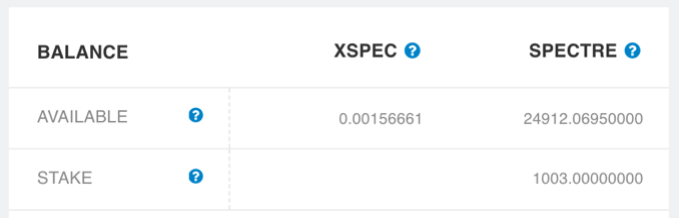
\includegraphics[width=0.5\textwidth]{Wallet-BalanceDualCoin.png} 
\end{figure}

 

The ‘dual-coin’ system can be seen as a feature allowing for complete transparent transactions and network audit functions if needed but without any privacy indebted overhead such as resource intensive calculations. Privacy maintaining SPECTRE can ONLY be created by consuming XSPEC at this time and the total supply on the network will always be transparent. There is no ‘bleed through’ between the two types of transaction outputs and no compromise in privacy.